
%$ currentsection
\section{Grids of Figures}
\begin{frame}
\tableofcontents[currentsection]
\end{frame}
%$

\subsection{Fourier Synthesis}
\begin{frame}[fragile]
\frametitle{Fourier Synthesis}
Given a \verb|freq| and a set of
\verb|components|, find the sum of
the harmonic sinusoids.
\snippet{py/fourier}
\end{frame}

% \subsection{Rectangular Waves}
\begin{frame}
\frametitle{Synthesis of Rectangular Waves}
\snippet{py/make_plots}
\end{frame}

\subsection{Grids of Figures}
\begin{frame}
\frametitle{Closeup of 1Hz Waves}
\vspace{-1em}
\begin{multicols}{2}
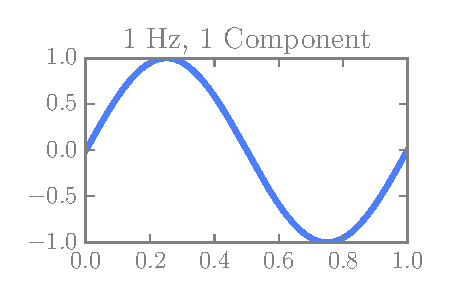
\includegraphics[width=\linewidth]{../img/fouriers/1_1.pdf}

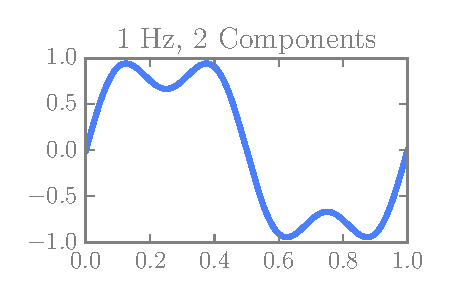
\includegraphics[width=\linewidth]{../img/fouriers/1_2.pdf}

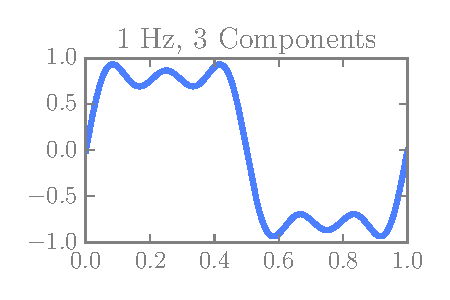
\includegraphics[width=\linewidth]{../img/fouriers/1_3.pdf}

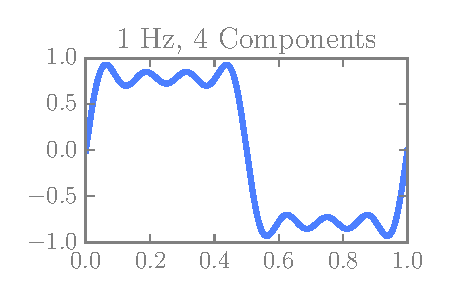
\includegraphics[width=\linewidth]{../img/fouriers/1_4.pdf}
\end{multicols}
\end{frame}

\begin{frame}
\frametitle{Varying Frequency and Harmonics}
\begin{multicols}{5}
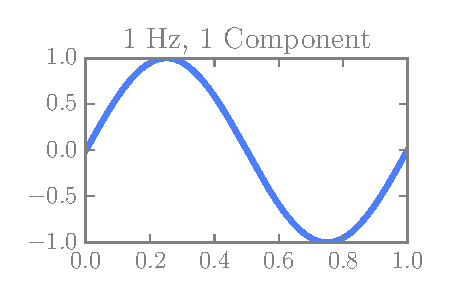
\includegraphics[width=\linewidth]{../img/fouriers/1_1.pdf}

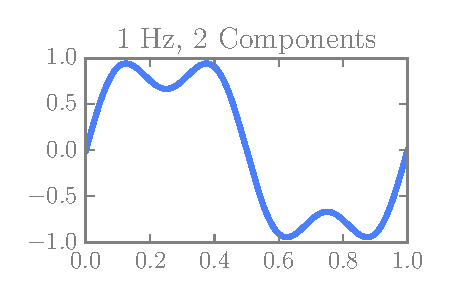
\includegraphics[width=\linewidth]{../img/fouriers/1_2.pdf}

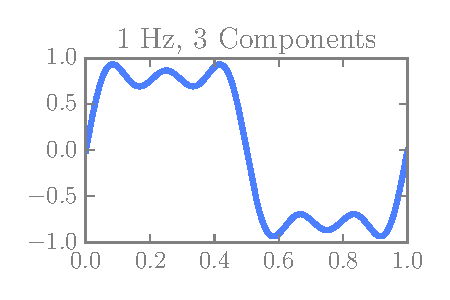
\includegraphics[width=\linewidth]{../img/fouriers/1_3.pdf}

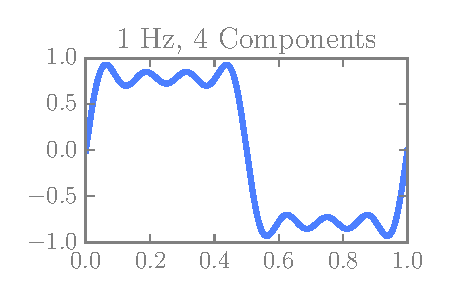
\includegraphics[width=\linewidth]{../img/fouriers/1_4.pdf}

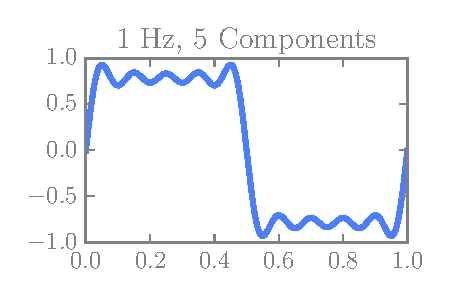
\includegraphics[width=\linewidth]{../img/fouriers/1_5.pdf}

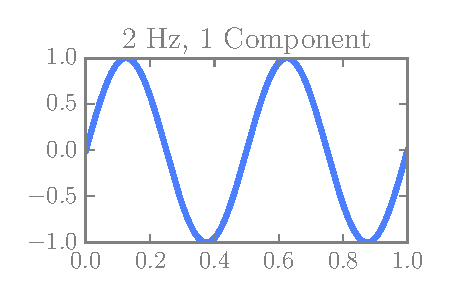
\includegraphics[width=\linewidth]{../img/fouriers/2_1.pdf}

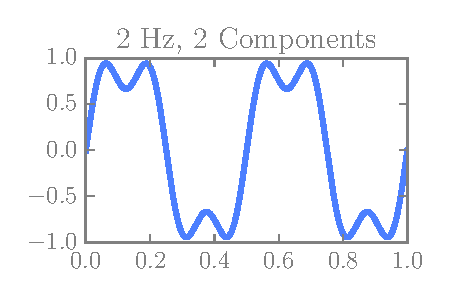
\includegraphics[width=\linewidth]{../img/fouriers/2_2.pdf}

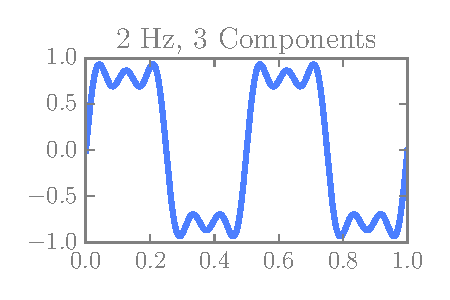
\includegraphics[width=\linewidth]{../img/fouriers/2_3.pdf}

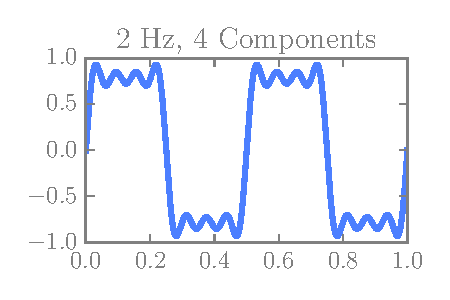
\includegraphics[width=\linewidth]{../img/fouriers/2_4.pdf}

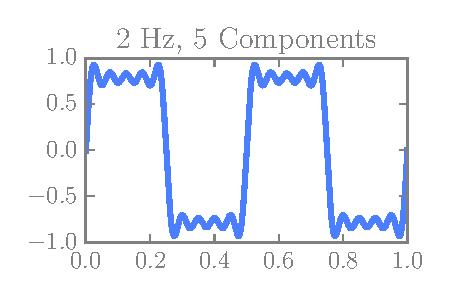
\includegraphics[width=\linewidth]{../img/fouriers/2_5.pdf}

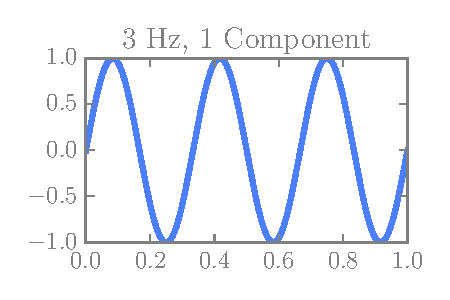
\includegraphics[width=\linewidth]{../img/fouriers/3_1.pdf}

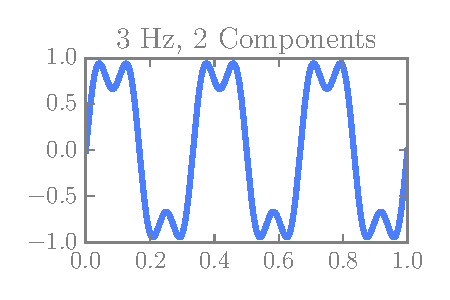
\includegraphics[width=\linewidth]{../img/fouriers/3_2.pdf}

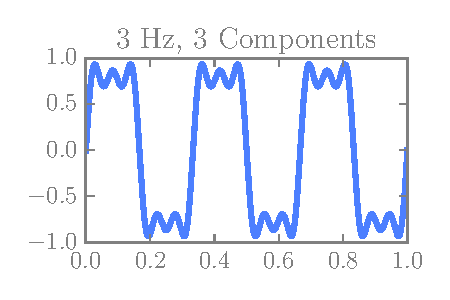
\includegraphics[width=\linewidth]{../img/fouriers/3_3.pdf}

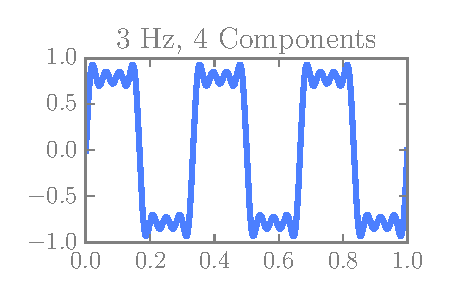
\includegraphics[width=\linewidth]{../img/fouriers/3_4.pdf}

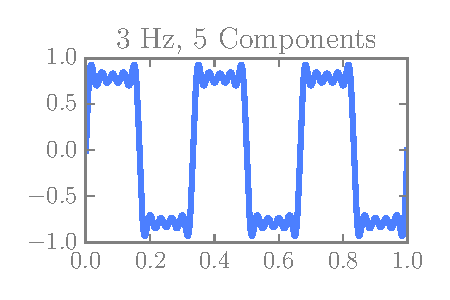
\includegraphics[width=\linewidth]{../img/fouriers/3_5.pdf}

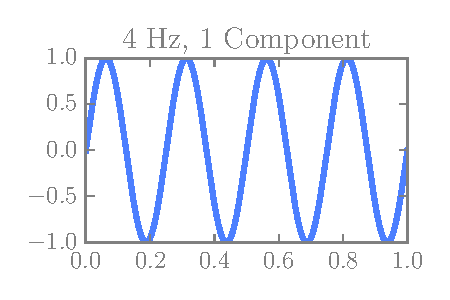
\includegraphics[width=\linewidth]{../img/fouriers/4_1.pdf}

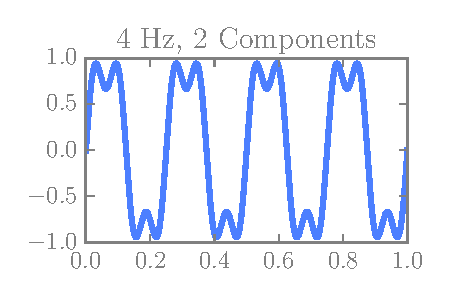
\includegraphics[width=\linewidth]{../img/fouriers/4_2.pdf}

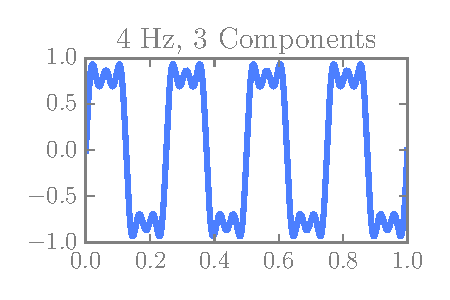
\includegraphics[width=\linewidth]{../img/fouriers/4_3.pdf}

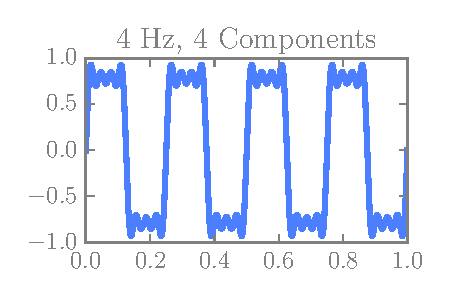
\includegraphics[width=\linewidth]{../img/fouriers/4_4.pdf}

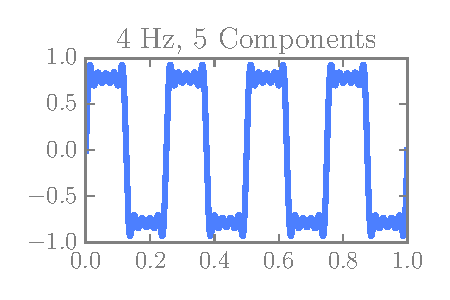
\includegraphics[width=\linewidth]{../img/fouriers/4_5.pdf}

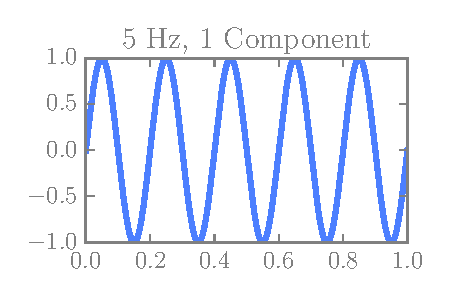
\includegraphics[width=\linewidth]{../img/fouriers/5_1.pdf}

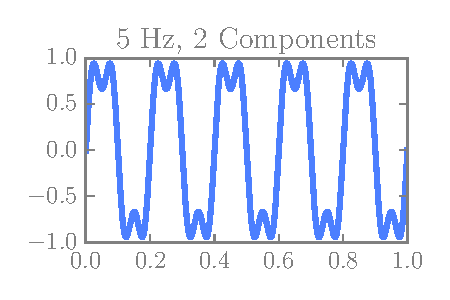
\includegraphics[width=\linewidth]{../img/fouriers/5_2.pdf}

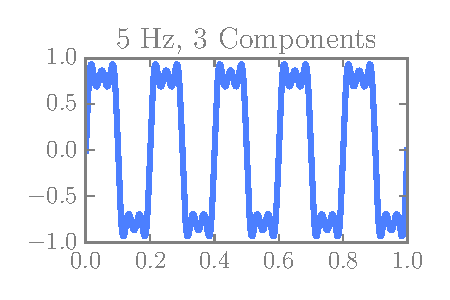
\includegraphics[width=\linewidth]{../img/fouriers/5_3.pdf}

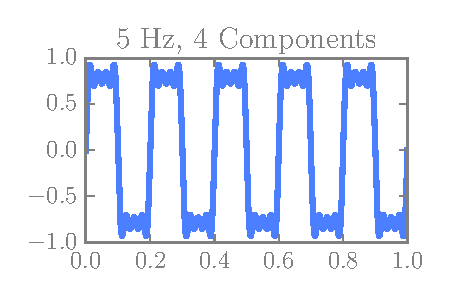
\includegraphics[width=\linewidth]{../img/fouriers/5_4.pdf}

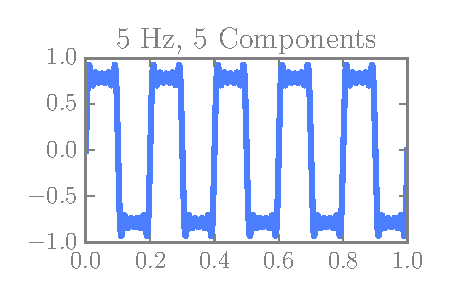
\includegraphics[width=\linewidth]{../img/fouriers/5_5.pdf}
\end{multicols}
\end{frame}

\begin{frame}
\frametitle{Using the Grid}
\snippet{py/using_grid}
\end{frame}

\begin{frame}
\frametitle{Writing the Grid}
\snippet{py/grid}
\end{frame}

\subsection{Templating}
\begin{frame}[fragile]
\frametitle{Pythong String Formatting}
\snippet{py/string_formatting}
Notice the curly brace differences in 
\verb|string1| and
\verb|string2|. Output is at the top
of the next slide. 
Compare against the standard 
\verb|printf| function.
\end{frame}

%$ template_results
\newcommand{\pageme}[1]{%
  \begin{minipage}[t][1em]{\linewidth}
  #1 \end{minipage}}   % verbatim
\begin{frame}[fragile] % troubles...
  \frametitle{Results!}
  \begin{tabular}{r | m{0.7\linewidth}}
  \verb|pieces/amiri.tex| & \pageme{%
  \verbatiminput{pieces/amiri.tex}} \\
  \verb|pieces/leev.tex| & \pageme{%
  \verbatiminput{pieces/leev.tex}} \\
  this slide's source & 
  \snippet{tex/template_results}
  \end{tabular}
\end{frame}
%$

\begin{frame}[fragile]
\frametitle{That {\bf template()} Function}
Define the sequence \verb|[=[var]=]| as an
indication that we want to insert the python
variable \verb|var| into a latex string.
\snippet{py/template}
\end{frame}

\begin{frame}
\frametitle{Templating Examples from UNOEF}
\centering

\includegraphics[width=0.4\paperwidth]{%
../img/EmirJoseMacari_2015_08_26.png}
\hspace{1em}

\includegraphics[height=0.7\paperheight]{%
../img/2015_07_08_IttiphongLeevongwat.png}
\end{frame}

\begin{frame}
\frametitle{Templating Examples from UNOEF}
\centering
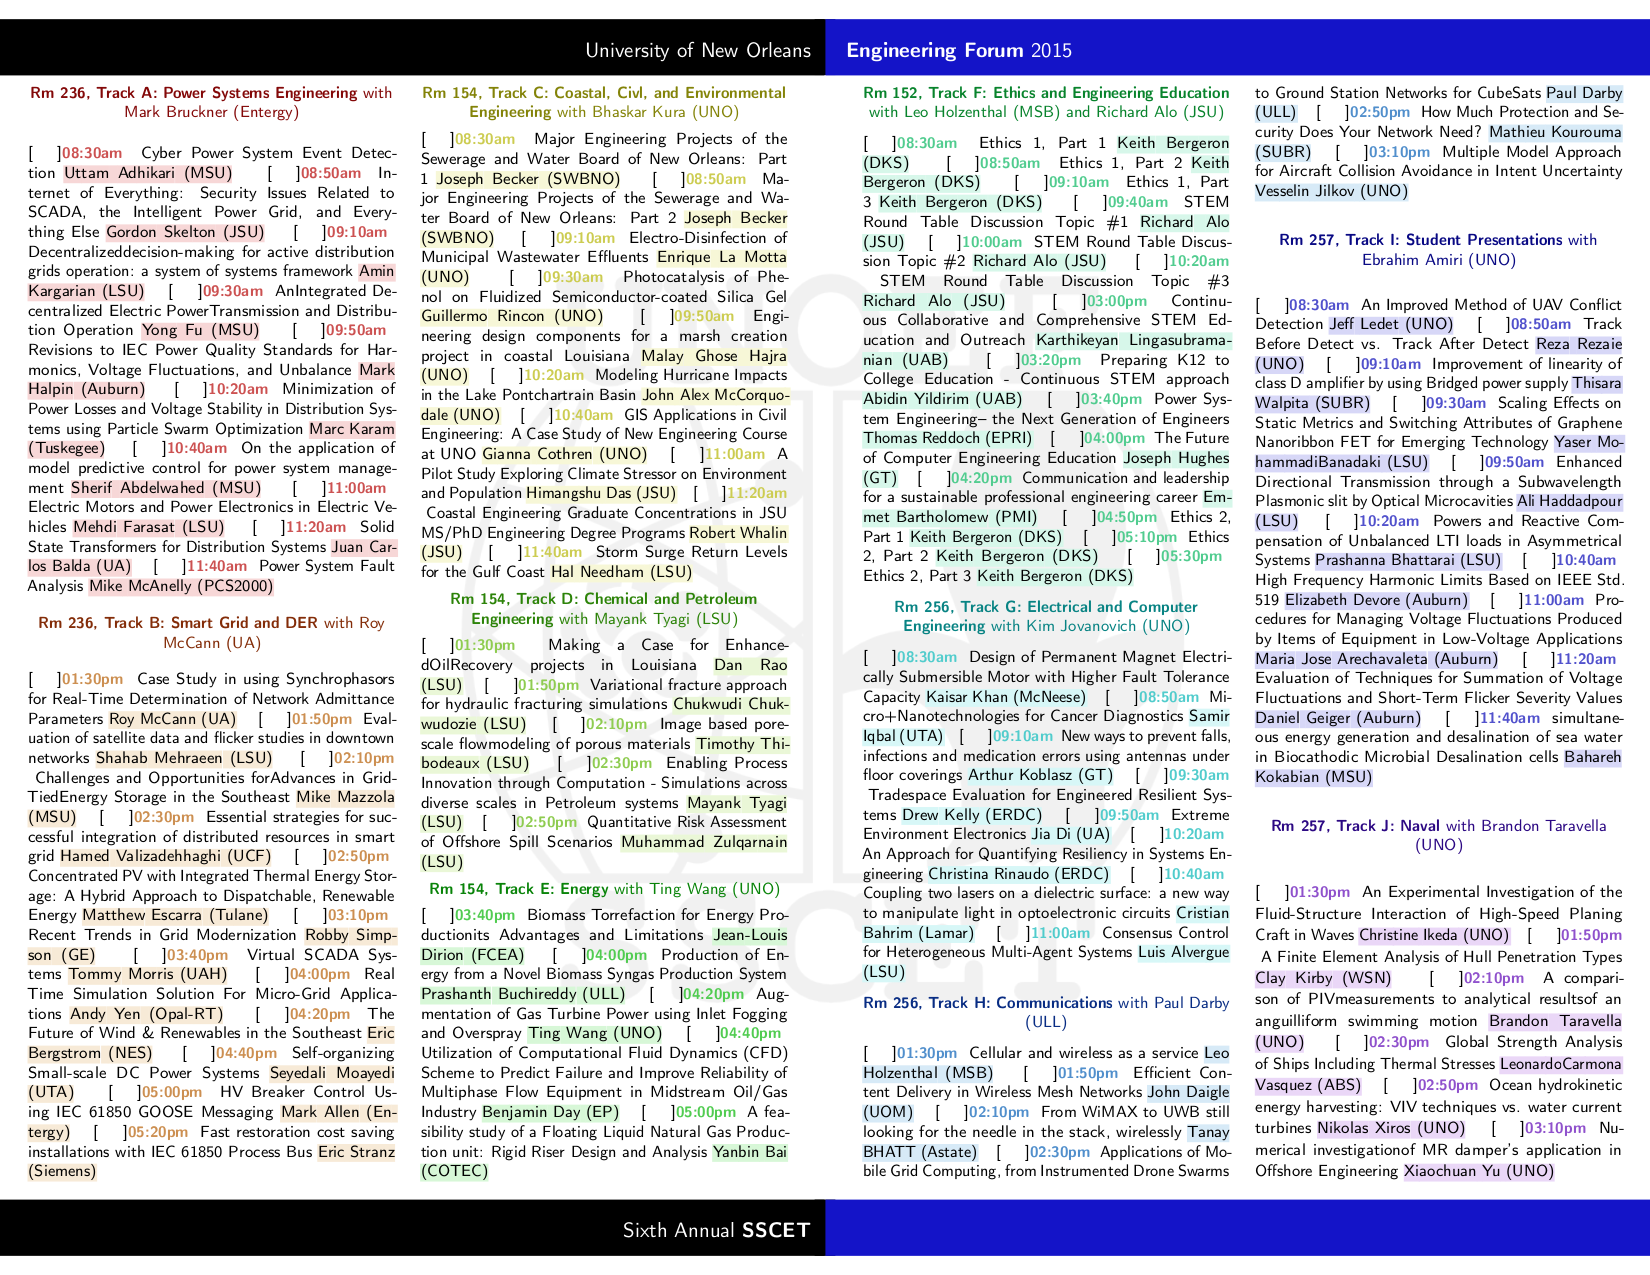
\includegraphics[height=0.7\paperheight]{%
../img/2015_UNOEF_Schedule.png}
\end{frame}

